\documentclass[border=10pt]{standalone}
\usepackage{pgfplots}
\pgfplotsset{compat=1.18}

\begin{document}
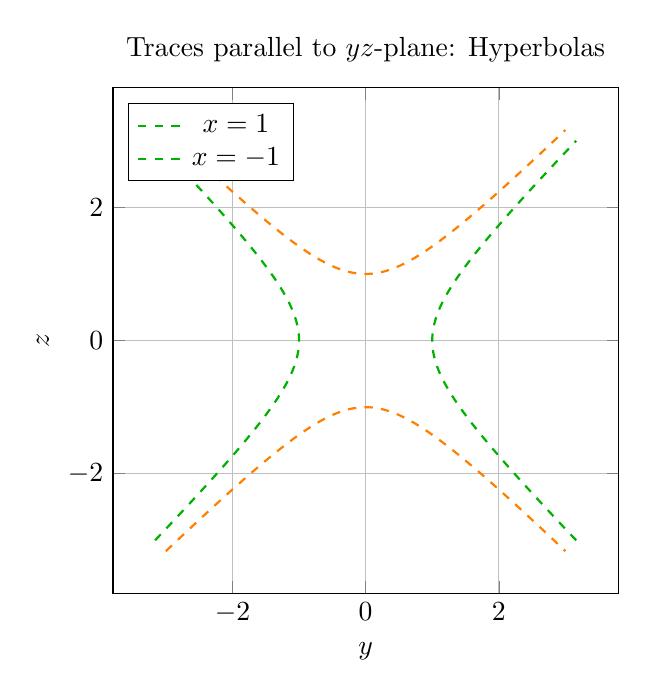
\begin{tikzpicture}
\begin{axis}[
    xlabel={$y$},
    ylabel={$z$},
    title={Traces parallel to $yz$-plane: Hyperbolas},
    grid=major,
    axis equal,
    width=8cm,
    height=8cm,
    domain=-3:3,
    legend pos=north west,
]
% x=1: y^2 - z^2 = 1 => y = +/- sqrt(1+z^2)
\addplot[green!70!black, dashed, thick, domain=-3:3, samples=100] ({sqrt(1+x^2)}, x);
\addplot[green!70!black, dashed, thick, domain=-3:3, samples=100] ({-sqrt(1+x^2)}, x);
\addlegendentry{$x=1$}

% x=-1: z^2 - y^2 = 1 => z = +/- sqrt(1+y^2)
\addplot[orange, dashed, thick, domain=-3:3, samples=100] (x, {sqrt(1+x^2)});
\addplot[orange, dashed, thick, domain=-3:3, samples=100] (x, {-sqrt(1+x^2)});
\addlegendentry{$x=-1$}
\end{axis}
\end{tikzpicture}
\end{document}